\chapter{Ergebnisse}
\label{sec:ergebnisse}



\vspace*{-2.5mm}
\renewcommand{\arraystretch}{1.2}
\begin{table}[h!]
	\centering 
	\caption{Messwerttabelle für den Praktikumsversuch Thermische Abfallbehandlung - Grundlagen}
	\resizebox{\textwidth}{!}{
	\begin{tabulary}{23cm}{l|c|c|c}
		\textbf{Daten} & \textbf{Einheit}  & \textbf{Vorher} & \textbf{Nachher} \\ 
		\hline  
	Masse Tiegel (TIC-Probe) & $\si{\gram}$ & 45,717 & 53,0574\\
	Masse TIC-Probe	& $\si{\gram}$ & 38,717 & 7,340\\
	Masse Tiegel (original Abfall)	& $\si{\gram}$ &28,4613 & 29,0690\\
	Masse original Abfall (zur Trocknung) & $\si{\gram}$ &2,976 & 2,878\\
	\cline{3-4}
	Trockensubstanz original Abfall & \text{Ma.-\%} & \multicolumn{2}{c}{96,71\%}  \\
	\cline{3-4}
	Masse org. Abfall (zur Verbrennung) & $\si{\gram}$ & 2,878& 2,203\\
	\cline{3-4}
	org. Trockensubstanz original Abfall &\text{Ma.-\%} &\multicolumn{2}{c}{ 18,96\% }  \\
	\hline
	\multicolumn{2}{c|}{\textbf{Messung TIC}}   & \textbf{Masse $\left[ \si{\gram} \right] $} & \textbf{Messergebnis $\left[ \si{\micro \volt
	\per \minute}  \right] $} \\
	\hline
	\multicolumn{2}{l|}{Abfallprobe 1 für TIC-Messung}  & 0,994& 40329,7\\
	\multicolumn{2}{l|}{Kalibrierpunkt 1 ($CaCO_3$)}  & 0,0618& 33472,8\\
	\multicolumn{2}{l|}{Kalibrierpunkt 2 ($CaCO_3$)}  & 0,073& 37642,8\\
	\multicolumn{2}{l|}{Abfallprobe 2 für TIC-Messung}  &0,999 & 55644,0\\
	\hline
	\multicolumn{2}{c|}{\textbf{Messung TC \& Cl}}   & \textbf{Masse $\left[ \si{\gram} \right] $} & \textbf{Messergebnis $\left[ \si{\gram\per\kilogram}\right] $ } \\
	\hline
	\multicolumn{2}{l|}{TC Blindwert (z.B. gebrannter Kalk)}  &0,2343 &4,11 \\
	\multicolumn{2}{l|}{TC orig. Abfall (nach Trocknung)}  &0,0790 & 274,26\\
	\multicolumn{2}{l|}{TC TIC-Mischprobe (nach Trocknung)}  & 0,4749& 43,85\\
	\multicolumn{2}{l|}{Chlorgehalt orig. Abfall (\SI{80}{\milli\liter} aus \SI{160}{\milli\liter})}  & - & 0,855 (0,085\%)\\
	\end{tabulary}
}
	\label{master_messwerttabelle}
\end{table}
\FloatBarrier
\vspace*{-2.5mm}
\renewcommand{\arraystretch}{1.2}

%\begin{table}[h!]
%	\centering 
%	%\resizebox{\textwidth}{!}{
%		\begin{tabulary}{23cm}{L|C|C}
%			\textbf{Messung TIC} & \textbf{Masse $\left[ \si{\gram} \right] $} & \textbf{Messergebnis $\left[ \si{\micro \volt
%					\per \minute}  \right] $} \\
%			\hline
%			Abfallprobe für TIC-Messung  & & \\
%			Kalibrierpunkt 1 ($CaCO_3$)  & & \\
%			Kalibrierpunkt 2 ($CaCO_3$) & & \\
%			%\multicolumn{1}{l}{Kalibrierpunkt 1 ($CaCO_3$)} & & & \\
%			\hline
%			\textbf{Messung TC \& Cl}  & \textbf{Masse $\left[ \si{\gram} \right] $} & \textbf{Messergebnis $\left[ \si{\gram\per\kilogram}\right] $ } \\
%			\hline
%			TC Blindwert (z.B. gebrannter Kalk) & & \\
%			TC orig. Abfall (nach Trocknung) & & \\
%			TC TIC-Mischprobe (nach Trocknung) & & \\
%			Chlorgehalt orig. Abfall %(\SI{80}{\milli\liter} aus \SI{160}{\milli\liter}) 
%			& & \\
%		\end{tabulary}
%	%}
%\end{table}
%\FloatBarrier

\newpage

\section{Bestimmung des TIC-Gehaltes}
\label{sec:tic}

Im folgenden Abschnitt sind die Messwerte für die Massen %$\left[\si{\gram}\right]$ 
der Müll- und der Carbonatproben aufgeführt, sowie deren per Software berechnetes Messergebnis $\left[\si{\micro \volt \per \minute}\right]$. Alle Werte für den TIC-Gehalt in Tabelle \ref{master_messwerttabelle} wurden vor der Trocknung der Proben aufgenommen.

\vspace*{-5mm}
\subsubsection{Bestimmung des Carbonatgehaltes $\boldsymbol{\chi}$ für Probe 1}
\begin{flalign}
	 	\frac{m_{\text{Abfall-Carbonat}}}{e_{\text{Abfall-Carbonat}}} &=	\frac{m_{\text{Carbonat}}}{e_{\text{Carbonat}}} \\[5pt]
		m_{\text{Abfall-Carbonat}} 		&= 	\frac{e_{\text{Abfall-Carbonat}}}{e_{\text{Carbonat}}}*m_{\text{Carbonat}}\\[5pt]
		m_{\text{Abfall-Carbonat}} 		&= \frac{\SI{40329,7}{\micro \volt \per \minute}}{\SI{33472,8}{\micro \volt \per \minute}}*\SI{0.0618}{\gram}\\[5pt]
		m_{\text{Abfall-Carbonat}} 		&= \underline{\SI{0.0745}{\gram}}\\[8pt]
		\chi_{\text{Abfall-Carbonat}} 	&= \frac{m_{\text{Abfall-Carbonat}}}{m_{\text{Abfall}}}\\[5pt]
		\chi_{\text{Abfall-Carbonat}} 	&= \frac{\SI{0.0745}{\gram}}{\SI{0.9940}{\gram}}\\[5pt]
		\chi_{\text{Abfall-Carbonat}} 	&= \underline{\underline{0,07494 \approx 7,5 \%}}
\end{flalign}

\subsubsection{Bestimmung des Carbonatgehaltes $\boldsymbol{\chi}$ für Probe 2}
\begin{flalign}
\frac{m_{\text{Abfall-Carbonat}}}{e_{\text{Abfall-Carbonat}}} &=	\frac{m_{\text{Carbonat}}}{e_{\text{Carbonat}}} \\[5pt]
m_{\text{Abfall-Carbonat}} 		&= 	\frac{e_{\text{Abfall-Carbonat}}}{e_{\text{Carbonat}}}*m_{\text{Carbonat}}\\[5pt]
m_{\text{Abfall-Carbonat}} 		&= \frac{\SI{55644,0}{\micro \volt \per \minute}}{\SI{33472,8}{\micro \volt \per \minute}}*\SI{0,0618}{\gram}\\[5pt]
m_{\text{Abfall-Carbonat}} 		&= \underline{\SI{0,1027}{\gram}}\\[8pt]
\chi_{\text{Abfall-Carbonat}} 	&= \frac{m_{\text{Abfall-Carbonat}}}{m_{\text{Abfall}}}\\[5pt]
\chi_{\text{Abfall-Carbonat}} 	&= \frac{\SI{0,1027}{\gram}}{\SI{0.9990}{\gram}}\\[5pt]
\chi_{\text{Abfall-Carbonat}} 	&= \underline{\underline{0,10284 \approx 10,3 \%}}
\end{flalign}

\vspace*{-5mm}

\subsubsection{Mittlerer Carbonatgehalt}
\begin{flalign}
	\chi_{\text{Abfall-Carbonat,mittel}} &= \frac{\chi_1+\chi_2}{2} = \frac{7,5\%+10,3\%}{2}\\[2mm]
										 &= \underline{\underline{8,9\%}}
\end{flalign}

\newpage

Die aufgenommenen Messergebnisse mit den zugehörigen Graphen des Computerprogramms lassen sich in den Abbildungen \ref{dia:k1} bis \ref{dia:m2} nachvollziehen.
%Start
\begin{figure}[h!]
	\centering
	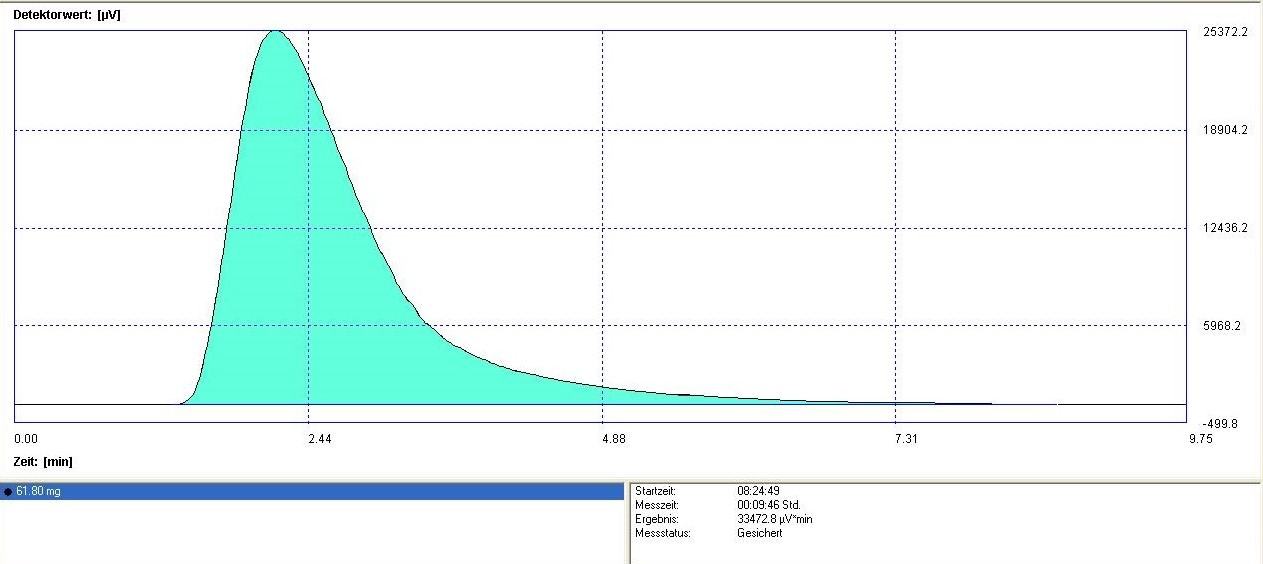
\includegraphics[width=0.59\textwidth]{img/CaCO3_k1}
	\caption{Messkurve 1 für Kalibrierung mit \ce{CaCO3}}
	\label{dia:k1}
\end{figure}
\FloatBarrier
%Ende

%Start
\begin{figure}[h!]
	\centering
	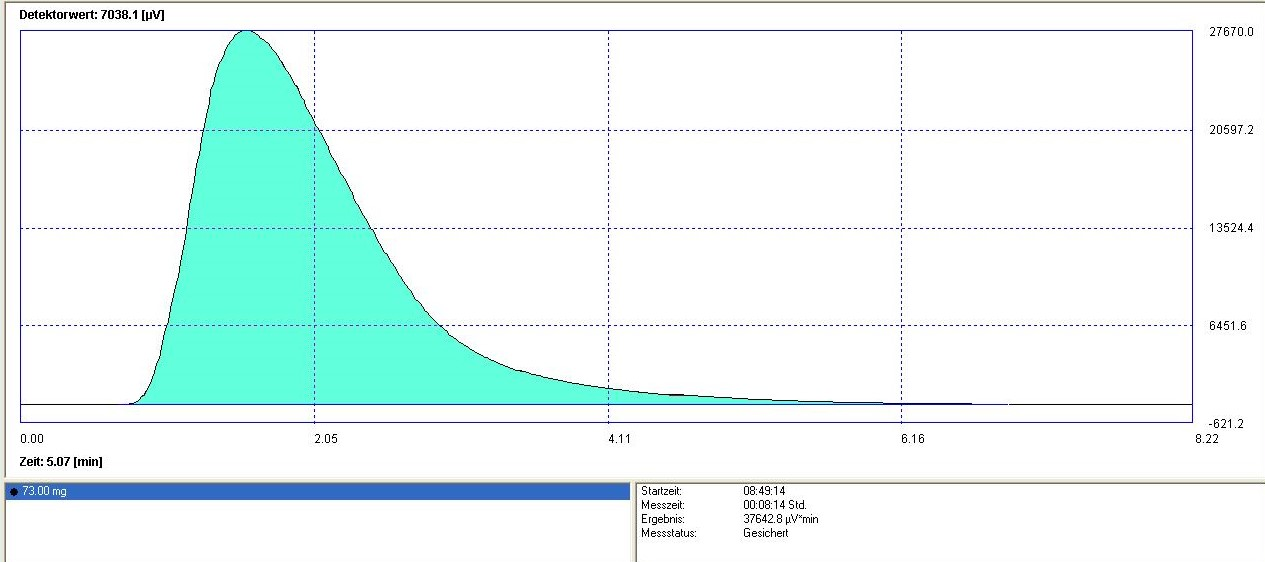
\includegraphics[width=0.59\textwidth]{img/CaCO3_k2}
	\caption{Messkurve 2 für Kalibrierung mit \ce{CaCO3}}
	\label{dia:k2}
\end{figure}
\FloatBarrier
%Ende

%Start
\begin{figure}[h!]
	\centering
	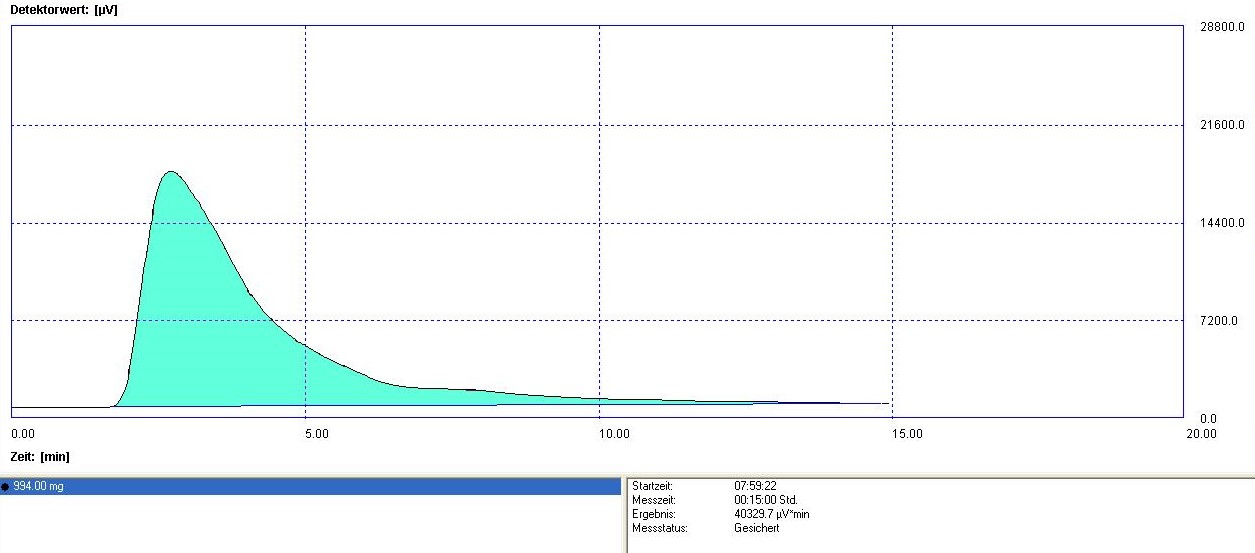
\includegraphics[width=0.59\textwidth]{img/Muell_V1}
	\caption{Messkurve für Müllprobe 1}
	\label{dia:m1}
\end{figure}
\FloatBarrier
%Ende

%Start
\begin{figure}[h!]
	\centering
	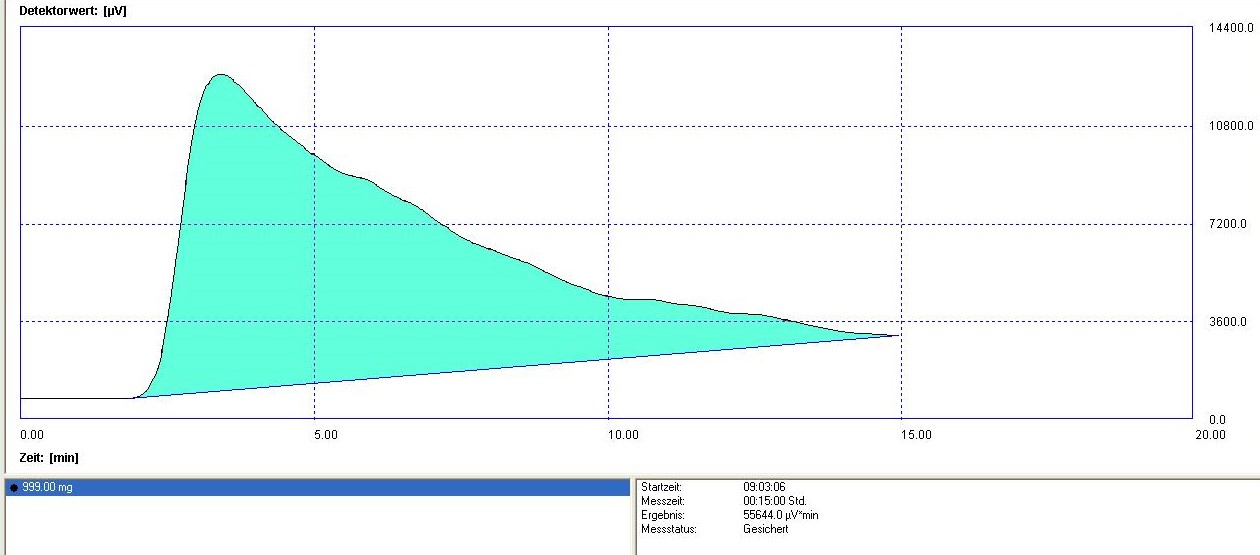
\includegraphics[width=0.59\textwidth]{img/Muell_V2}
	\caption{Messkurve für Müllprobe 2}
	\label{dia:m2}
\end{figure}
\FloatBarrier
%Ende

\newpage

Um die Messwerte im Vergleich zu den Blindproben beurteilen zu können sind diese im Diagramm \ref{dia:kalibrierkurve} aufgezeigt und werden mittels Abweichungsrechnung ab Gleichung \ref{gl:abweichung} weiter analysiert.

\begin{figure}[h!]
	\begin{center}
		\begin{tikzpicture}
		\begin{axis}[
		xlabel={$m \left[\si{\milli \gram}\right]$},
		ylabel={$\Phi \left[\si{\micro \volt \minute}\right]$},
		xmin = 0,
		xmax = 120,
		width= 15cm,
		height=7cm,
		ymin=0,
		ymax=70000,
		axis x line=bottom,
		axis y line=left,
		legend style={
			at={(0.2,-0.25)},anchor=north west}]
		
		\addplot [domain=0:200, samples=101,dotted]{540.24*x + 54.501};
		\addlegendentry{Verlauf der Messdaten $(540,24*x + 54,50)$};
		%\addplot [domain=0:200, samples=101,dashed]{476.91*x + 3876.1};
		\addplot [domain=0:200, samples=101,]{524.41*x + 141.53};
		\addlegendentry{Kalibrierkurve $(524,41*x + 141,53)$};
		\addplot+ [mark=*, color=black] coordinates {(74.55,40329.7)};
		\addlegendentry{\ce{CaCO3}-Müllprobe 1};
		\addplot [mark=*, color=black] coordinates {(102.9,55644.0)};
		\addlegendentry{\ce{CaCO3}-Müllprobe 2};
		\addplot [mark=x, color=blue, only marks] coordinates {(61.8,33472.8) (73.0,37642.8) (0,0)};
		\addlegendentry{\ce{CaCO3}-Blindproben};
		
		\addplot [mark=x, color=red] coordinates {(74.5,40329.7)};
		\addlegendentry{Kalibrierpunkt (berechnet)};
		\end{axis}%
		\end{tikzpicture}%
	\end{center}
	\caption{Kalibrierkurve zur Bestimmung des Carbonatgehaltes der \\  Müllprobe 2}
	\label{dia:kalibrierkurve}
\end{figure}
\FloatBarrier


\subsubsection{Abweichung von Kalibrierkurve}

\begin{flalign}
\label{gl:abweichung}
	a	&= \frac{\Phi_{Mess}-\Phi_{Kali}}{\Phi_{Kali}}\\[2mm]
	a_1	&= \frac{\SI{40329.7}{\micro \volt \minute}-\SI{39236,30
		}{\micro \volt \minute}}{\SI{39236,30
	}{\micro \volt \minute}} = \underline{\underline{2,8\%}}\\[2mm]
	a_2	&= \frac{\SI{55644.0}{\micro \volt \minute}-\SI{54101,75}{\micro \volt \minute}}{\SI{54101,75
		}{\micro \volt \minute}} = \underline{\underline{2,9\%}}
\end{flalign}

\newpage

\section{Bestimmung des TC}
\label{sec:tc}
\subsubsection{Bestimmung des TC der originalen Abfallprobe über Mittelwertbildung}
Berechnung mit mittlerem Carbonatgehalt ($TIC$) und Glühverlust ($TOC$):
\begin{flalign}
	TC	&= TIC+TOC\\
		&= 8,9\%+23,5\% = 32,4\%\\
		&= \frac{\SI{32,4}{\gram}}{\SI{100}{gramm}}=\frac{\SI{324}{\gram}}{\SI{1000}{gramm}}\\
		&\approx \underline{\SI{324}{\gram \per \kg}}
\end{flalign}

Berechnung mit mittlerem Carbonatgehalt (TIC) und vorbehandelter TIC Probe mit TC-Analyse (TOC):
\begin{flalign}
TC	&= TIC+TOC\\
	&= \SI{89}{\gram \per \kg}+\SI{43,85}{\gram \per \kg}\\
	&\approx \underline{\SI{133}{\gram \per \kg}}
\end{flalign}

Mittelwert beider Herangehensweisen:
\begin{flalign}
	TC 	&= \frac{\SI{133}{\gram \per \kg}+\SI{324}{\gram \per \kg}}{2}\\[2mm]
		&= \underline{\underline{\SI{228,5}{\gram \per \kg} \quad (22,85\%)}}
\end{flalign}
\FloatBarrier

Analog dazu ergab die direkte Messung mittels \textit{Analysegerät} einen Wert von \SI{274,26}{\gram \per \kg} für den $TC$.
\vspace*{-5mm}
\begin{figure}[h!]
\renewcommand{\arraystretch}{1.2}
	\centering
	\caption{Daten zum TC-Gehalt}
	\begin{tabular}{c|c|c||c}
	\hline
	\textbf{TOC mit Glühverlust} & \textbf{TOC mit Analysegerät} & \textbf{Mittelwert} & \textbf{Analysegerät} \\
	\hline
	\SI{324}{\gram \per \kg} & \SI{133}{\gram \per \kg} & \SI{228,5}{\gram \per \kg} & \SI{274,26}{\gram \per \kg}\\
	\hline
	 32,4 \% & 13,3 \% & 22,85 \% & 27,43 \%\\
	\hline
	\end{tabular}
\end{figure}
\FloatBarrier

\vspace*{-5mm}
\begin{figure}[h!]
	\renewcommand{\arraystretch}{1.2}
	\centering
	\caption{Daten zu den Kohlenstoffgehalten}
	\label{tab:tc}
	\begin{tabular}{c|c|c||c}
		\hline
		\textbf{Kohlenstofftyp} & \textbf{Messwert 1} & \textbf{Messwert 2} & \textbf{Mittelwert}  \\
		\hline
		TOC		&	23,45\%		& 4,39\%	& $\approx 14\%$\\
		TIC		&	7,5\%		& 10,3\%	& $\approx 9\%$ \\
		TC		&	22,85\%		& 27,43\%	& $\approx 25\%$ \\
		\hline
	\end{tabular}
\end{figure}
\FloatBarrier

\newpage

\section{Bestimmung von Brenn- und Heizwert}
In diesem Abschnitt werden die Berechnungen und Ergebnisse zur Bestimmung der Trockensubstanz $TS$, des Wassergehaltes $W$, sowie des Glühverlustes $GV$ dargestellt. \\
Brenn- und Heizwert wurden mittels Näherungsformeln nach \textsc{Shin} bestimmt und geben Auskunft über die Wertigkeit der Müllprobe als Ersatzbrennstoff. Für die Berechnung wurden die Ergebnisse aus Tabelle \ref{tab:ts_w_gv} genutzt.

\subsubsection{Bestimmung des Trockensubstanzgehalt $\mathbf{TS}$} 
\begin{flalign}
TS \left[\%\right]	&= \frac{m_{\text{Trockensubstanz}}}{m_\text{gesamt}}*100\%\\
TS_{\text{TIC}}		&= \frac{\SI{7,340}{\gram}}{\SI{38,717}{\gram}}*100\%\\
&=\underline{18,96\%}\\[2mm]
TS_{\text{org.}}		&= \frac{\SI{2,878}{\gram}}{\SI{2,976}{\gram}}*100\%\\
&=\underline{96,71\%}
\end{flalign}

\subsubsection{Bestimmung des Wassergehaltes $\mathbf{W}$} 
%Trockensubstanz TIC = 38,717 dann 7,340
%TS original = 2,976 dann 2,878
\begin{flalign}
W \left[\%\right]	&= \frac{m_\text{gesamt}-m_{\text{Trockensubstanz}}}{m_\text{gesamt}}*100\%\\
W_{\text{TIC}}		&= \frac{\SI{38,717}{\gram}-\SI{7,340}{\gram}}{\SI{38,717}{\gram}}*100\%\\
&=\underline{81,04\%}\\[2mm]
W_{\text{org.}}		&= \frac{\SI{2,976}{\gram}-\SI{2,878}{\gram}}{\SI{2,976}{\gram}}*100\%\\
&=\underline{3,29\%}
\end{flalign}

\subsubsection{Bestimmung des Glühverlustes $\mathbf{GV}$}
%VERBENNUNG
\begin{flalign}
GV \left[\%\right]				&= \frac{m_{\text{gesamt}}-m_{\text{Glührückstand}}}{m_\text{gesamt}}*100\%\\[2mm]
GV_{\text{org.}} &= \frac{\SI{2,878}{\gram}-\SI{2,203}{\gram} }{\SI{2,878}{\gram}}*100\%\\
&= \underline{\SI{23,45}{\percent}}
\end{flalign}

\subsubsection{Bestimmung des Inertstoffgehaltes $\boldsymbol{IS}$}
%VERBENNUNG
\begin{flalign}
IS\left[\%\right]				&= \SI{100}{\percent}-TC-W\\
IS_{\text{org.}} &\approx \SI{100}{\percent}-\SI{25}{\percent}-\SI{3}{\percent}\\
&\approx \underline{\SI{72}{\percent}}
\end{flalign}

%Tabelle START
\vspace*{-.5cm}
\renewcommand{\arraystretch}{1.2}
\begin{table}[h!]
	\centering
	\caption{Daten zu Trockensubstanz, Wassergehalt, Glühverlust und Inertstoffgehalt \\ der Müllprobe 2}
	\label{tab:ts_w_gv}
	%\resizebox{10cm}{!}{
	\begin{tabulary}{1.2\textwidth}{C|CC|CC}
		\hline
		\textbf{Probe} & \textbf{Trockensubstanz} & \textbf{Wassergehalt} & \textbf{Glühverlust} & \textbf{Inertstoffgehalt}\\ 
		\hline
		Original & 96,71\% & 3,29\% & 23,45\%&76,55\%\\
		Nach TIC & 18,96\% & 81,04\% & - & -\\
		\hline
	\end{tabulary}
	%}
\end{table}
\FloatBarrier
\vspace*{-2.5mm}
%Tabelle Ende

\subsubsection{Bestimmung des Brennwertes $\mathbf{H_s}$}
\begin{flalign}
	H_s \left[\si{\kilo \joule \per \kg}\right]		&= 523*GV^{0,77}\\
	H_s(org.)	&= 523*23,45^{0,77}\\	
				&= \underline{\underline{\SI{5936,24}{\kilo \joule \per \kg}\approx\SI{5,94}{\mega \joule \per \kg}\approx\SI{1,65}{\kWh \per \kg}}}
\end{flalign}


\subsubsection{Bestimmung des Heizwertes $\mathbf{H_i}$} 
\begin{flalign}
H_i	\left[\si{\kilo \joule \per \kg}\right]	&= H_s*\frac{TS}{100}-25*\left(0,09*H*TS+W\right)\\
											&= H_s*\frac{TS}{100}-25*\left(0,09*\frac{GV}{15}*TS+W\right)\\[2mm]
H_i(org.)		&= \SI{5936,24}{\kilo \joule \per \kg}*\frac{96,71}{100}-25*\left(0,09*\frac{23,45}{15}*96,71+3,29\right)\\
				&= \underline{\underline{\SI{5318,51}{\kilo \joule \per \kg}\approx\SI{5,32}{\mega \joule \per \kg}\approx\SI{1.48}{\kWh \per \kg}}}
\end{flalign}
 
